\documentclass[UTF8,a4paper,11pt,fontset=fandol]{ctexart}
\usepackage[margin=22mm,headheight=14pt]{geometry}
\usepackage{amsmath,amssymb,booktabs,graphicx,xcolor,fancyhdr,enumitem,hyperref,longtable,xurl}
\setlength{\emergencystretch}{3em}
\definecolor{ink}{HTML}{183B37}\definecolor{accent}{HTML}{216B62}
\hypersetup{colorlinks=true,urlcolor=accent,linkcolor=accent,pdftitle={梁鉴技术补充：推导、实验与复现},pdfauthor={}}
\pagestyle{fancy}\fancyhf{}\fancyhead[L]{\small 梁鉴 / 技术补充与内部实验佐证}\fancyhead[R]{\small 2026-10-13}\fancyfoot[C]{\thepage}
\ctexset{section={format=\Large\bfseries\color{ink}},subsection={format=\normalsize\bfseries\color{ink}}}
\setlist{itemsep=2pt,topsep=3pt}\linespread{1.12}\newcommand{\HybridMAE}{0.135}
\newcommand{\PhysicsMAE}{0.150}
\newcommand{\AIMAE}{0.757}
\newcommand{\HybridTime}{21.6}
\newcommand{\PhysicsTime}{81.7}
\newcommand{\AITime}{3.9}
\newcommand{\Speedup}{3.78}
\newcommand{\CallSaving}{80.2}
\newcommand{\Coverage}{87.5}
\newcommand{\Width}{2.08}
\newcommand{\Accept}{97.5}
\newcommand{\HealthyFalseAblation}{44.2}
\newcommand{\MeshMAE}{0.128}
\newcommand{\TripleMAE}{4.77}
\newcommand{\MassMAE}{5.51}
\newcommand{\NoiseMAE}{0.801}
\newcommand{\FullSeconds}{128.8}
\newcommand{\HybridDamagedMAE}{0.517}

\begin{document}
\section*{1\quad 模型、假设与可辨识性}
本文件是可复现实验的内部技术佐证，不是第三方检测报告、专利证明或用户应用证明。所有数值均来自合成数据。两页主报告按官方大纲整理，此处保留必要推导与失败边界。
\subsection*{1.1\quad 梁模型与边界}
采用线弹性、小变形、细长悬臂梁。忽略剪切变形、转动惯性、阻尼、夹持柔度和材料非均匀性。长度$L=1.2$\,m，截面$b=0.03$\,m、$h=0.006$\,m，$A=bh$，$I=bh^3/12$；$E=70\times10^9$\,Pa，$\rho=2700$\,kg/m$^3$。6个等长损伤区，每区2个单元，左端位移与转角固定。

一个长度$\ell$的Euler--Bernoulli单元，其自由度为$[w_1,\theta_1,w_2,\theta_2]^\mathsf T$。由三次Hermite插值$w=Nq$，弹性能$U=\frac12\int EI(w'')^2dx$及动能$T=\frac12\int\rho A\dot w^2dx$得到：
\begin{align*}
K_e&=\frac{EI}{\ell^3}\begin{bmatrix}12&6\ell&-12&6\ell\\6\ell&4\ell^2&-6\ell&2\ell^2\\-12&-6\ell&12&-6\ell\\6\ell&2\ell^2&-6\ell&4\ell^2\end{bmatrix},\\
M_e&=\frac{\rho A\ell}{420}\begin{bmatrix}156&22\ell&54&-13\ell\\22\ell&4\ell^2&13\ell&-3\ell^2\\54&13\ell&156&-22\ell\\-13\ell&-3\ell^2&-22\ell&4\ell^2\end{bmatrix}.
\end{align*}
按节点连接组装后删除左端两个自由度，解广义对称特征值问题。令第$j$区局部刚度折减$d_j$、整体刚度因子$\alpha$，则$K=\alpha\sum_j(1-d_j)K_j^0$。这里损伤不改变质量，也不代表裂纹深度的直接估计。
\subsection*{1.2\quad 环境混淆的严格边界}
若所有分区$d_j=c$，则$K=(1-c)\alpha K_0$。对任意$c$和$\alpha$，仅凭模态不能区分均匀损伤与整体模量变化。进一步，$K$统一乘以$\alpha$时，$\omega_r$乘以$\sqrt\alpha$，归一化振型不变。这解释了频率变化不能单独作为局部损伤证据。

本项目通过“最多两处损伤，其他区域健康”的稀疏支持集约束确定参考刚度。它是使用条件，不是从测试中发现的普适定律。三处损伤和附加质量因此被专门列为失配测试。
\subsection*{1.3\quad 单位与量纲}
位移$m$、转角$rad$、力$N$、弯矩$N\cdot m$分别与平移/转动自由度共轭，单元矩阵不同分块的单位随自由度而异，不能将所有刚度项统称为$N/m$。$E$为$N/m^2$、$I$为$m^4$、$\rho A$为$kg/m$；特征值为$s^{-2}$，$f=\omega/(2\pi)$为Hz。损伤$d$、因子$\alpha$、对数频率比和归一化振型均无量纲。
\newpage
\section*{2\quad AI--力学融合算法}
\subsection*{2.1\quad 观测与学习}
在$x/L=1/6,\ldots,1$采样振型，用梁端值归一化并固定符号；按频率升序对应前五阶模态。观测向量为5个$\log(f_r/f_r^0)$与30个归一化振型分量，共35维。前三阶的3个频率与18个振型分量用于拟合，后两阶的2个频率与12个振型分量保留作检查。

噪声在模态特征层注入：对数频率标准差0.001、归一化振型标准差0.003，相互独立。它是便于控制变量的简化观测模型；包括参考端坐标在内的噪声并未模拟从原始传感器波形归一化后产生的相关误差。实物应用应重新识别噪声结构和权重。

Extra Trees使用160棵树、最小叶节点样本数2、全部输入特征、单线程，随机种子11/29/47。标签为六区损伤和$\log\alpha$。输出损伤评分最高的三个分区，组成$\varnothing$、三个单区、三个双区共7个支持集。取前三个是预设的算力与召回折中，并未用测试结果调参。
\subsection*{2.2\quad 有界反演与支持集选择}
对每个支持集$S$，令集外损伤为零，求解
\[
\mathrm{RSS}_S=\min_{d_S,\log\alpha}\sum_{i\in\mathcal I}\big[(g_i(d,\alpha)-y_i)/\sigma_i\big]^2,
\]
并计算$\mathrm{RSS}_S+(|S|+1)\log21$。在独立高斯特征噪声和已知尺度的简化模型下，该式对应忽略公共常数的BIC形式；不将其解释为严格的支持集后验概率。$d\in[0,0.65]$，$\alpha\in[0.65,1.35]$；候选均采用SciPy有界最小二乘，每候选最多35次函数迭代，实际内部有限差分前向调用另计。

融合方案以AI结果初始化。穷举基线枚举全部$1+6+\binom62=22$个支持集，以损伤0.12、$\alpha=1$初始化。两者均为局部连续优化；“穷举”指位置组合全部遍历，不是对连续参数全局最优的证明。初始化不同是方法组成，不能把全部速度差归于候选数比。
\subsection*{2.3\quad 区间与独立模态}
对每种子独立120个校准样本，计算最大分区误差$s_i=\max_j|\hat d_{ij}-d_{ij}|$。令$k=\lceil(n+1)(1-\beta)\rceil$、$q=s_{(k)}$，$\beta=0.1$，输出$[\hat d_j-q,\hat d_j+q]\cap[0,0.65]$。取最大分数使目标为六个分区同时覆盖。标准分割共形结论依赖校准与新样本交换性；有限测试集实测覆盖可偏离90\%，不保证筛选后子集或分布外覆盖。

另计算留出残差$R=\sqrt{\frac1{14}\sum_{i\in\mathcal H}[(g_i-y_i)/\sigma_i]^2}$，阈值为校准集的95\%有限样本分位数。$R$超阈值时提示复核；未超阈值不是工程安全证明。这一校核不使用测试真值，也不回流修正拟合参数。
\newpage
\section*{3\quad 实验设计与误差口径}
每种子独立生成2400训练、120校准和240测试。健康、单损伤、双损伤的抽样概率为0.2、0.5、0.3；损伤位置均匀无放回抽取，程度均匀分布于$[0.08,0.45]$，整体因子均匀分布于$[0.88,1.12]$。无复制同一损伤样本加噪后再跨集合划分。
\begin{center}\small\begin{tabular}{p{25mm}p{113mm}}\toprule
测试域 & 相对于常规域的变更（每域3种子$\times$40例）\\\midrule
常规域 & 与训练分布相同，样本随机流独立\\
健康环境变化 & 全部分区损伤为0，仍有整体刚度变化与噪声\\
三倍噪声 & 频率与振型噪声标准差同时乘3，算法权重不作适配\\
加密网格 & 用24单元生成、12单元识别；仍采用粗网格健康频率作为观测参考\\
三处损伤 & 恰好3区损伤，超出候选模型最多2区的限制\\
附加质量 & $x/L=2/3$处加入总梁质量3\%--8\%的点质量，反演未包含该变量\\\bottomrule
\end{tabular}\end{center}
算法固定在首次正式测试前；预检仅用于力学测试和运行成本判断，正式三组种子的训练/校准/测试均重新生成。没有使用外部斑图、预训练生成模型或真实桥梁数据。

全区MAE为$\frac{100}{6N}\sum_{i,j}|\hat d_{ij}-d_{ij}|$，单位为百分点，不是相对于真实损伤的百分比误差。健康区较多，因此同时报告仅受损区的MAE，避免平均值掩盖受损区误差。损伤判别阈值固定为0.05；定位F1按全部分区微平均，完全匹配率要求每例全部6个分区的判别均正确。健康域单独报告误报率，不用没有阳性类别的F1论证能力。

耗时采用同机单线程墙钟时间；融合耗时含AI推理和全部候选反演，纯AI更快。离线训练/校准不含在在线加速比内，整套流程耗时\FullSeconds\,s；不同硬件和并发负载会改变该值。前向调用数提供更稳定的开销证据。三组种子而非720个模型重复，不能以样本数冒充训练重复数。
\begin{center}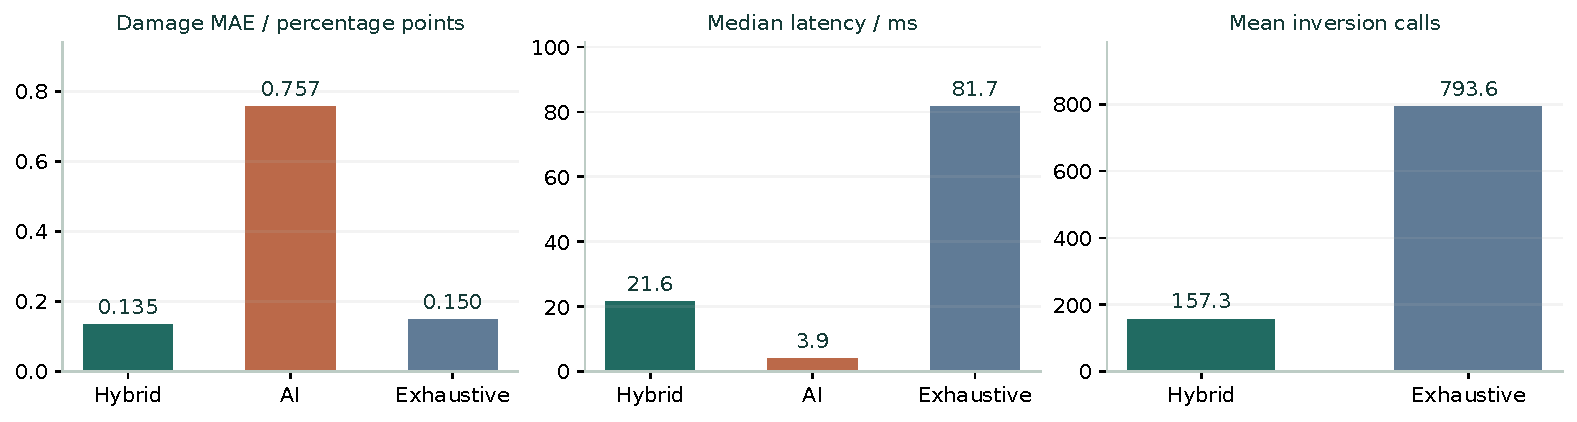
\includegraphics[width=\linewidth]{generated/headline.pdf}\end{center}
\begin{center}\scriptsize\begin{tabular}{lrrrr}\toprule
常规域方法 & 全区MAE/百分点 & 受损区MAE/百分点 & 定位F1 & 中位耗时/ms\\\midrule
AI+力学校核 & 0.135 & 0.517 & 1.000 & 21.6 \\
纯AI & 0.757 & 2.639 & 0.992 & 3.9 \\
穷举物理反演 & 0.150 & 0.524 & 1.000 & 81.7 \\
不估计环境（消融） & 3.248 & 10.644 & 0.667 & 53.5 \\
\bottomrule\end{tabular}
\end{center}
常规域融合方案与穷举物理基线的误差差值较小，未开展足以支持精度优越性的统计检验。主要主张是此次设定下误差接近，同时减少在线反演工作量。无损环境消融用于说明因素必要性，不能替代对强基线的比较。
\newpage
\section*{4\quad 泛化、拒判与失败分析}
\begin{center}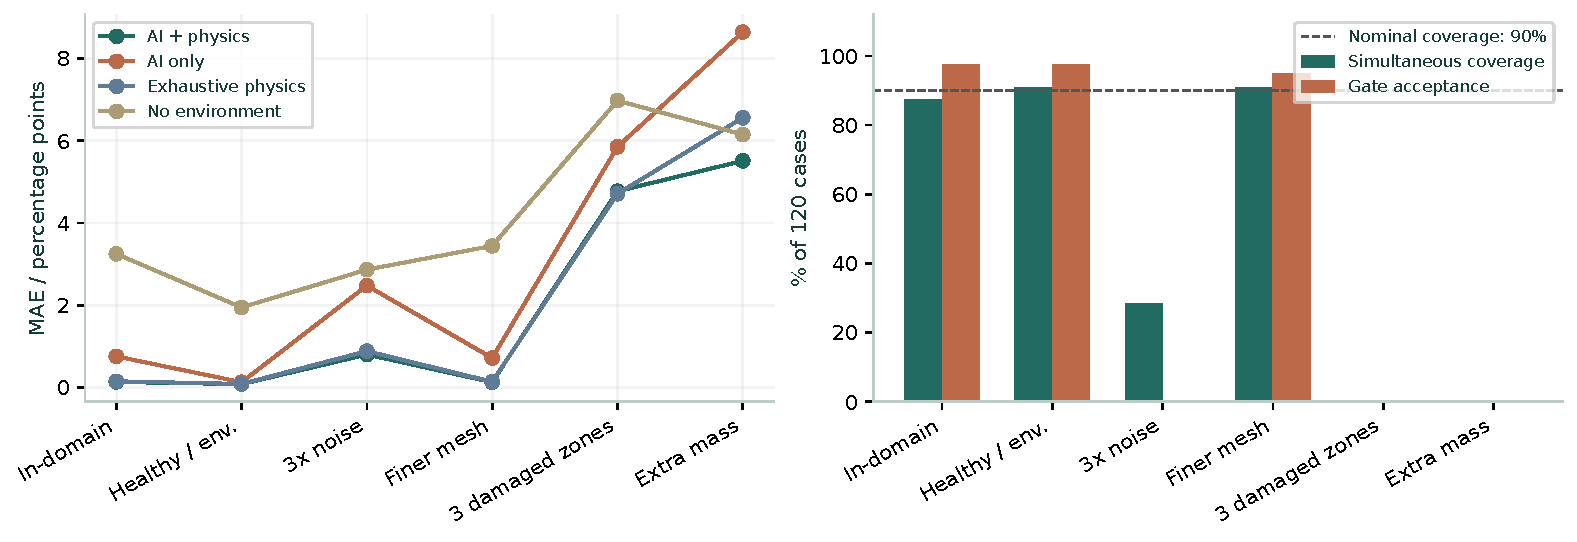
\includegraphics[width=\linewidth]{generated/robustness.pdf}\end{center}
\begin{center}\small\begin{tabular}{lrrrr}\toprule
测试域（各120例） & MAE/百分点 & 定位完全匹配/\% & 区间覆盖/\% & 校核接受/\%\\\midrule
常规域 & 0.135 & 100.0 & 87.5 & 97.5 \\
健康环境变化 & 0.082 & 100.0 & 90.8 & 97.5 \\
三倍噪声 & 0.801 & 79.2 & 28.3 & 0.0 \\
加密网格 & 0.128 & 100.0 & 90.8 & 95.0 \\
三处损伤 & 4.771 & 0.0 & 0.0 & 0.0 \\
附加质量 & 5.510 & 14.2 & 0.0 & 0.0 \\
\bottomrule\end{tabular}
\end{center}
常规域90\%区间实测覆盖率\Coverage\%，低于名义值；网格迁移与健康子域覆盖率另列。不能将某个有限测试集没有达到90\%直接改写为“校准失效”，也不能凭交换性理论将实测值改成90\%。每个新部署场景都需要新的校准数据与覆盖监测。

三倍噪声组全区误差\NoiseMAE 个百分点，三处损伤组\TripleMAE 个百分点，附加质量组\MassMAE 个百分点。三类组均被留出残差触发复核，表明在这批较明显的扰动上校核有用。微弱、恶意构造或与损伤等效的失配仍可能通过校核，本实验未建立最坏情况保障。

三处损伤的完全定位匹配率为0符合模型上限，不能被其较高的微平均F1掩盖。附加质量可能造成健康梁被误判为损伤，说明反演结果在失配下不可直接使用。UI仍展示估计数值以便分析，同时醒目标注需要复核。
\begin{center}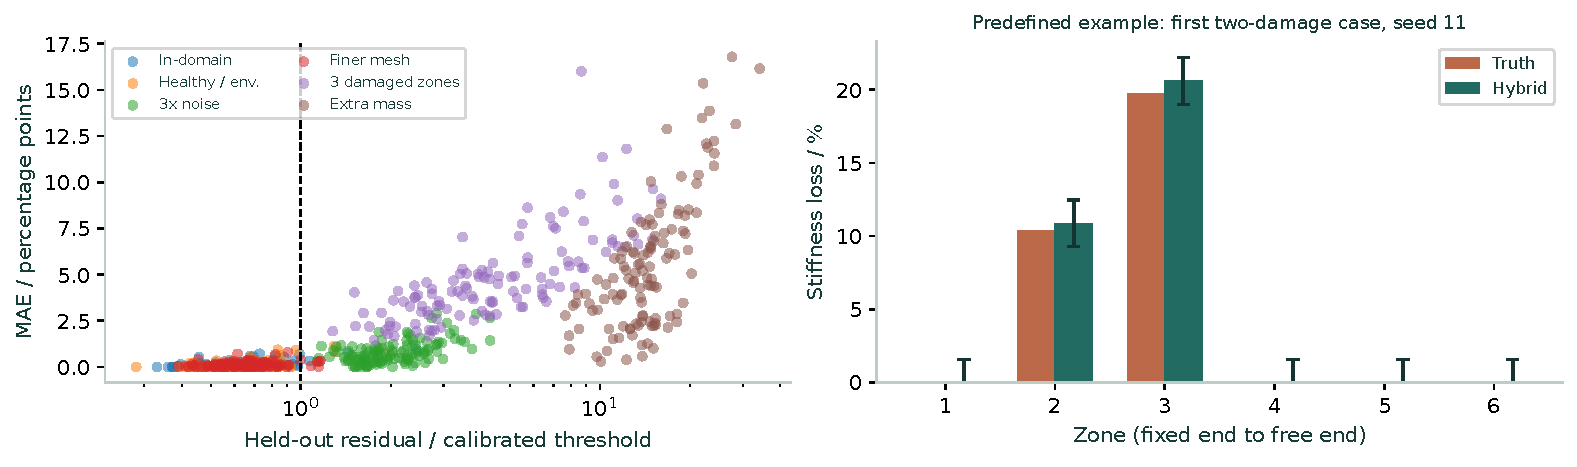
\includegraphics[width=\linewidth]{generated/diagnostics.pdf}\end{center}
右侧示例为种子11中按生成顺序找到的第一个双损伤常规样本，并非按最低误差筛选。左侧包含所有720个融合预测，横轴为留出残差与阈值之比，虚线右侧提示复核。区间与门限都仅由校准集确定。
\newpage
\section*{5\quad 验证、运行与真实应用边界}
\subsection*{5.1\quad 力学与数值验证}
\begin{enumerate}
\item 无损悬臂梁解析频率：$f_r=\frac{\lambda_r^2}{2\pi L^2}\sqrt{EI/(\rho A)}$。前五根依次为1.875104、4.694091、7.854757、10.995541和14.137168；24单元相对误差低于$2\times10^{-4}$。
\item 端部单位力挠度$L^3/(3EI)$与数值解相对误差低于$10^{-9}$。
\item 检查$K\phi-M\phi\omega^2$残差、$M$正交、环境因子平方根缩放及均匀损伤不可辨识性。
\item 无噪声双损伤反演、候选数量、留出特征隔离、共形有限样本分位数和非法输入检查。
\item 12/24/48单元的损伤梁频率逐级收敛；原始数值见\texttt{results/validation.json}。共10项测试全部通过。
\end{enumerate}
两次从头重建数据并训练，所有2880条预测除墙钟耗时外完全一致；全部数据数组与校准JSON一致。数据跨集合无完全重复观测，所有预测有界、优化器选中解均正常终止。上述结果不能证明所有实现路径无误，但分别覆盖解析解、数值稳定性、数据隔离与复现。
\subsection*{5.2\quad 复现入口}
在项目根目录创建Python环境，安装\texttt{requirements.txt}，依次运行：
\begin{quote}\ttfamily\small
python -m pytest tests -q\\
python scripts/study.py --output results/run1\\
python scripts/study.py --output results/run2\\
python scripts/verify.py\\
python scripts/present\_results.py\\
python demo/server.py --port 18766
\end{quote}
训练前设置单线程环境变量：
\begin{quote}\ttfamily\small OPENBLAS\_NUM\_THREADS=1\\OMP\_NUM\_THREADS=1\end{quote}
依赖版本与运行机器记入\texttt{provenance.json}。模型为joblib格式，仅加载本项目可信模型文件。展示层使用估计参数重新求模态并按单元Hermite形函数插值，动画为缩放变形示意，不代表实际振幅或实时振动频率。
\subsection*{5.3\quad 实物试验与团队工作}
下一步先在已知健康梁上核验夹持、质量和模态对应，再实施独立的局部刚度变化工况。记录原始波形、温度、传感器质量、夹持长度、采样率及重复测量。用固定参考通道统一移动测量的相位。完成健康模型校验后才能评估损伤；不能用附加质量替代已知刚度折减标签。

建议由队内分别承担模型/算法复核、数据试验、材料答辩；实际成员和责任人尚未提供，不能将建议分工写成已完成团队工作。本地算法与报告由Codex辅助生成，须由参赛者独立理解、审阅与确认。
\newpage
\section*{6\quad 来源、原创边界与材料清单}
本项目未复制GitHub候选仓库的源代码或结果。标准梁单元、Extra Trees、BIC与共形预测均为已有方法。自主实现贡献是针对六分区梁问题的模型、候选支持集耦合、校核流程、实验与可视化。创新程度应结合相关工作审慎评价，不能称为全球首创。
\begin{enumerate}[leftmargin=2em]
\item Peeters B, Maeck J, De Roeck G. Vibration-based damage detection in civil engineering: excitation sources and temperature effects. Smart Materials and Structures, 2001. \url{https://doi.org/10.1088/0964-1726/10/3/314}。作为环境混淆问题的需求依据。
\item Angelopoulos A N, Bates S. A Gentle Introduction to Conformal Prediction and Distribution-Free Uncertainty Quantification. 2021. \url{https://arxiv.org/abs/2107.07511}。作为分割校准与覆盖边界的依据。
\item scikit-learn，ExtraTreesRegressor。\url{https://scikit-learn.org/stable/modules/generated/sklearn.ensemble.ExtraTreesRegressor.html}。直接运行依赖，BSD-3-Clause。
\item SciPy，least\_squares与eigh。\url{https://docs.scipy.org/doc/scipy/reference/optimize.html}。有界优化和特征分解直接依赖。
\item pyfe3d。\url{https://github.com/saullocastro/pyfe3d}。3D有限元调研候选，BSD-3-Clause许可证快照保留；未纳入代码。参考仓库HEAD：\par\nolinkurl{d82c8fbb568e37bebbb69e47486fd1455492fed8}。
\item pycba。\url{https://github.com/ccaprani/pycba}。连续梁调研候选，仓库显示AGPL-3.0；未纳入代码。
\item Structural Health Monitoring Python。\url{https://github.com/alokpalai/structural-health-monitoring-python}。问题路线调研，页面未见明确许可证，因此未复制代码或数据。
\end{enumerate}
\subsection*{材料与单一数据来源}
\begin{center}\small\begin{tabular}{ll}\toprule
文件/目录 & 内容\\\midrule
\texttt{src/beam.py} & 力学求解、支持集反演、数据生成\\
\texttt{scripts/study.py} & 训练、校准、全域实验\\
\texttt{results/run1/data.npz} & 训练、校准、测试全部原始数组\\
\texttt{results/run1/records.json} & 每例真值、预测、残差、耗时、状态\\
\texttt{results/run1/model\_*.joblib} & 三组训练模型\\
\texttt{results/run2/} & 完整重训复算结果\\
\texttt{paper/generated/} & 从结果自动生成的表、数值宏、图\\
\texttt{demo/} & 本地交互演示与服务\\
\texttt{docs/AI\_USE.md} & AI使用范围与待人工核验事项\\\bottomrule
\end{tabular}\end{center}
匿名材料未填写学校、导师或LOGO。队号与队名等待补齐；本地材料不等于网盘上传或大赛平台接收。任何后续改模必须重新执行验证、更新论文数值并重算归档哈希。
\end{document}
